\chapter{Test Journal: Disturbance Frequency} \label{app:Disturbance}

\textbf{Date: 10/05/2017}

\subsection*{Purpose}
Find the frequency of the wave forces that affects the vessel. The wave forces can be modeled as a sinusoidal curve with a given frequency, unlike wind forces which are modeled as a constant force. To do this the vessel is left stationary in water and the effects of the waves are recorded. The frequency of the waves are determined by processing the data.

\subsection*{Equipment}
\begin{itemize}
    \item Vessel with all its components. 
    \item External laptop.
\end{itemize}

\subsection*{Procedure}
\begin{enumerate}
    \item Turn on all equipment.
    \item Remotely log into the vessel, when both, laptop and vessel's computer, are in the same network.
    \item Run the following nodes
    \begin{itemize}
        \item \lstinline[style=cinline]{/sensor_node}
    \end{itemize}
    \item Place the vessel in water without actuating the vessel.
    \item Record the following topics
    \begin{itemize}
        \item \lstinline[style=cinline]{/imu}      
    \end{itemize}
    \item Stop the recording after some time has passed.
    \item Turn off the equipment.
    \item Process the data.
\end{enumerate}

\subsection*{Results}
The Fast Fourier Transform (FFT) of $x_\mathrm{acc}$ was performed, as shown in \autoref{fig:waveDisturbance} thus the frequency of the disturbances can be seen as $f = 0.833 \mathrm{Hz}$.
%
\begin{figure}[H]
   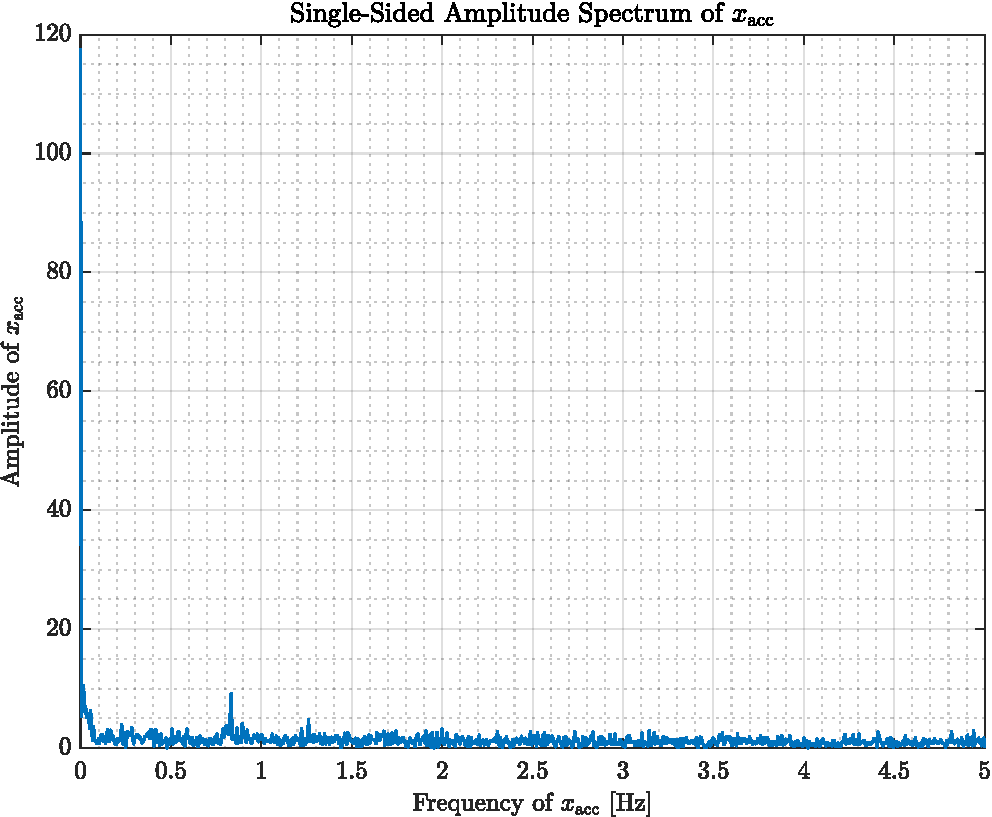
\includegraphics[width=.7\textwidth]{figures/waveDisturbance}
   \caption{FFT of $x_\mathrm{acc}$}
   \label{fig:waveDisturbance}
\end{figure}
%%
%\begin{flalign}
%    \sigma_{x\mathrm{n,GPS}}^2 & = 0.00050346 \ \mathrm{m}^2  \nonumber \\
%    \sigma_{y\mathrm{n,GPS}}^2 & = 0.00057036 \ \mathrm{m}^2  \nonumber
%\end{flalign}